\documentclass[12pt]{ximera}

\usepackage{nopageno}
\usepackage{amsmath}
\usepackage{graphicx}
\usepackage{geometry}
\geometry{top=1in,bottom=1in,right=0.75in,left=0.75in}
\usetikzlibrary{patterns}

\usepackage{fancyhdr}
\usepackage{lastpage}
 
\pagestyle{fancy}
\fancyhf{}
\rhead{\textsf{Form A}}
\lhead{\textsf{Calculus Knowledge Assessment v3}}
\rfoot{\textsf{Page \thepage\ of \pageref{LastPage}}}


\usepackage{multicol}
\setlength{\columnsep}{2cm}

\usepackage{enumitem}

\setitemize{noitemsep,topsep=0pt,parsep=0pt,partopsep=0pt}

\renewenvironment{multipleChoice}
{\begin{trivlist}\item[\hskip\labelsep\small\bfseries Choose the best answer:]
\hfil\begin{enumerate}\begin{multicols}{2}}
 {\end{multicols}\end{enumerate}\end{trivlist}}

\def\image{\begin{center}}
\def\endimage{\end{center}}

%\renewcommand{\choice}[2][]{\item \begin{minipage}[t]{2in}#2\end{minipage}\ifthenelse{\boolean{#1}}{\ifhandout \else \quad\checkmark\fi}{}}
\renewcommand{\choice}[2][]{\item \begin{minipage}[t]{2in}#2\end{minipage}\ifthenelse{\boolean{#1}}{\ifhandout \else  \fi}{}}


\begin{document}
\vspace{6ex}

\begin{minipage}{\textwidth}
\begin{problem}

  Four equally spaced numbers are shown below on a number line.
  \begin{image}
    \begin{tikzpicture}[x=0.19\textwidth]
      \draw[-{>[scale=1.75]}] (-0.05\textwidth,0) -- (0.8\textwidth,0);
      \foreach \x in {0,...,4} {%
        \draw (\x,-.1) -- (\x,.1);
        \node[anchor=north,yshift=-2pt] at (\x,0) {$\x$};
      }
      \draw (0.5,0) node [circle,fill,inner sep=1pt,label=above:$x$](e){};
      \draw (1.5,0) node [circle,fill,inner sep=1pt,label=above:$y$](e){};
      \draw (2.5,0) node [circle,fill,inner sep=1pt,label=above:$z$](e){};
      \draw (3.5,0) node [circle,fill,inner sep=1pt,label=above:$w$](e){};
    \end{tikzpicture}
  \end{image}
  Let $f(t) = t^2$ and consider $f(x)$ and $f(y)$ and $f(z)$ and $f(w)$.  Which pair of numbers is farthest apart?
  \begin{multipleChoice}
    \choice{The pair $f(x)$ and $f(y)$.}
    \choice{The pair $f(y)$ and $f(z)$.}
    \choice[correct]{The pair $f(z)$ and $f(w)$.}
    \choice{These pairs are all equally far apart}
  \end{multipleChoice}
\end{problem}
\end{minipage}

\vspace{6ex}

\begin{minipage}{\textwidth}
\begin{problem}

  Consider the following graph of a function, $f$, as seen through this
  window frame.  What can we say about $f(1)$?
  \begin{image}
    \includegraphics[scale= 0.25]{window}\\
  \end{image}
  \begin{multipleChoice}
    \choice{$f(1)=3$.}
    \choice{$f(1)$ is defined but we do not know it's value.}
    \choice{$f(1)$ is not defined.}
    \choice[correct]{We don't know anything about $f(1)$.}
  \end{multipleChoice}
\end{problem}
\end{minipage}

\vspace{6ex}

\begin{minipage}{\textwidth}
\begin{problem}
  %\GoodQuestions{Subject: Continuity and the Intermediate Value Theorem 4Q}
  You know the following statement is true: ``If $f$ is a
    polynomial function, then $f$ is a continuous function.''  Which
    of the following must also be true?
  \begin{multipleChoice}
     \choice[correct]{If $f$ is not continuous, then it is not a polynomial.}
     \choice{If $f$ is continuous, then it is a polynomial.}
     \choice{If $f$ is not a polynomial, then it is not continuous.}
     \choice{None of the above.}
  \end{multipleChoice}
\end{problem}
\end{minipage}

\vspace{6ex}

\begin{minipage}{\textwidth}
\begin{problem}
  %\GoodQuestions{Subject: Tangents, velocities, and other rates of change 2P}
  What can be said about the line tangent to the graph of $f(x)=x$ at $(0,0)$?
  \begin{multipleChoice}
  \choice{It is $y=0$.}
  \choice{It is $y=1$.}
  \choice[correct]{It is $y=x$.}
  \choice{It does not exist.}
  \choice{It is not unique. There are infinitely many tangent lines.}
  \end{multipleChoice}
\end{problem}
\end{minipage}

\vspace{6ex}

\begin{minipage}{\textwidth}
\begin{problem}
  %\recommendation{Elizabeth}
  % I fixed this to mention "at the origin"
  Suppose you are driving a car and you accelerate from a stopped
  position (at the origin) to 60 mph with a constant acceleration.
  Which graph below best resembles your position as a function of time
  over this time interval?
 
  \begin{multipleChoice}
    % increasing, concave up
    \choice[correct]{\begin{tikzpicture}[scale=0.33]\begin{axis}[clip=false,domain=0:1,ymin=-0.1,ymax=1.1,xmin=-0.1,xmax=1.1,xtick=\empty,ytick=\empty,axis lines=center,axis on top] \addplot [very thick, smooth] {x^2};\end{axis}\end{tikzpicture}}
    % increasing, concave down
    \choice{\begin{tikzpicture}[scale=0.33]\begin{axis}[clip=false,domain=0:1,ymin=-0.1,ymax=1.1,xmin=-0.1,xmax=1.1,xtick=\empty,ytick=\empty,axis lines=center,axis on top] \addplot [very thick, smooth,domain=0:1] ({x^2},{x});\end{axis}\end{tikzpicture}}
    % decreasing, concave down
    \choice{\begin{tikzpicture}[scale=0.33]\begin{axis}[clip=false,domain=0:1,ymin=-0.1,ymax=1.1,xmin=-0.1,xmax=1.1,xtick=\empty,ytick=\empty,axis lines=center,axis on top] \addplot [very thick, smooth,domain=0:1] ({x},{1-x^2});\end{axis}\end{tikzpicture}}
    % decreasing, concave up
    \choice{\begin{tikzpicture}[scale=0.33]\begin{axis}[clip=false,domain=0:1,ymin=-0.1,ymax=1.1,xmin=-0.1,xmax=1.1,xtick=\empty,ytick=\empty,axis lines=center,axis on top] \addplot [very thick, smooth,domain=0:1] ({x^2},{1-x});\end{axis}\end{tikzpicture}}
  \end{multipleChoice}
\end{problem}
\end{minipage}

\vspace{6ex}

\begin{minipage}{\textwidth}
\begin{problem}

  The graph of the position of an object with respect to time is given
  by a straight line with a positive slope.  What can we say about the
  acceleration of the object?
  \begin{multipleChoice}
    \choice{It is positive.}
    \choice{It is negative.}
    \choice[correct]{It is zero.}
    \choice{The acceleration changes from negative to positive.}
    \choice{We cannot say anything about the sign of the acceleration.}
  \end{multipleChoice}
\end{problem}
\end{minipage}

\vspace{6ex}

\begin{minipage}{\textwidth}
\begin{problem}
  
  Suppose $x$ is a number near one thousand, and $y$ is a number near $10^{10}$.  Which number below is nearest $x + y$?
  \begin{multipleChoice}
    \choice{$1000$}
    \choice[correct]{$10^{10}$}
    \choice{$10^{100}$}
    \choice{$10^{1000}$}
    \choice{$10^{1010}$}
  \end{multipleChoice}
\end{problem}
\end{minipage}

\vspace{6ex}

\begin{minipage}{\textwidth}
\begin{problem}

  Shown below is the graph of $y = e^x$ and a tangent line $y = mx + b$ to the graph passing through the point $(8,e^8)$.
  \begin{image}
    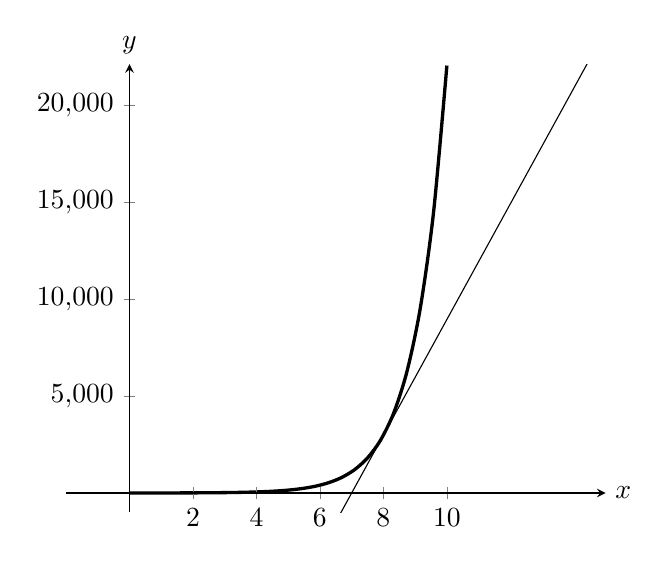
\begin{tikzpicture}
      \begin{axis}[
        clip=true,
        domain=0:10,
        ytickmin=0,ytickmax=20000,
        xtickmin=0,xtickmax=10,
        ymin=-1000, ymax=22100,
        xmin=-2, xmax=15,
        ytick={5000,10000,15000,20000},
        scaled y ticks=false,
        xlabel=$x$, ylabel=$y$,
        axis lines=center,
        every axis y label/.style={at=(current axis.above origin),anchor=south},
        every axis x label/.style={at=(current axis.right of origin),anchor=west},
        axis on top,
        ]          
        \addplot [very thick,smooth] {exp(x)};
        \addplot [smooth,domain=0:15] {exp(8)*(x-8) + exp(8)};
      \end{axis}
    \end{tikzpicture}  
  \end{image}
  How does $200m + b$ compare to $e^{200}$?
  \begin{multipleChoice}
    \choice{$200m + b$ equals $e^{200}$.}
    \choice{$200m + b$ is bigger than $e^{200}$.}
    \choice{$200m + b$ is a little bit smaller than $e^{200}$.}
    \choice[correct]{$200m + b$ is much smaller than $e^{200}$.}
  \end{multipleChoice}
\end{problem}
\end{minipage}

\vspace{6ex}

\begin{minipage}{\textwidth}
\begin{problem}

  Suppose $x$ is a positive number close to zero, and $y$ is a very large number.  What can be said about $y/x$?
  \begin{multipleChoice}
    \choice[correct]{It is very large.}
    \choice{It is close to zero.}
    \choice{It is very negative.}
    \choice{It could be very positive or very negative.}
  \end{multipleChoice}
\end{problem}
\end{minipage}

\vspace{6ex}

\begin{minipage}{\textwidth}
\begin{problem}
  Suppose $a$ and $b$ and $A$ and $B$ are very large, positive numbers, and suppose $A > a$ and $B < b$.  How does $A/B$ compare to $a/b$?
  \begin{multipleChoice}
    \choice[correct]{$A/B$ is bigger than $a/b$}
    \choice{$A/B$ is equal to $a/b$}
    \choice{$A/B$ is smaller than $a/b$}
    \choice{It could be that $A/B$ or $a/b$ is larger}
  \end{multipleChoice}
\end{problem}
\end{minipage}

\vspace{6ex}

\begin{minipage}{\textwidth}
\begin{problem}
  Suppose $f$ is a differentiable function and $f(0) = 0$ and
  $f(\sin 0.03) = 6$.  What is a best guess for $f(0.01)$?
  \begin{multipleChoice}
    \choice[correct]{$2$}
    \choice{$4$}
    \choice{$6$}
  \end{multipleChoice}
\end{problem}
\end{minipage}

\vspace{6ex}

\begin{minipage}{\textwidth}
\begin{problem}
  Suppose $x, y, z$ are positive quantities which are depend on time
  $t$.  If $xyz = 1$ and $x$ is increasing, what must be true of $y$ and $z$?
  \begin{multipleChoice}
    \choice{$y$ must be increasing}
    \choice{$y$ must be decreasing}
    \choice{$z$ must be increasing}
    \choice{$z$ must be decreasing}
    \choice[correct]{None of these statements are necessarily true}
  \end{multipleChoice}
\end{problem}
\end{minipage}

\vspace{6ex}

\begin{minipage}{\textwidth}
\begin{problem}
  Suppose the slope of a tangent line to the graph of $f$ at the point $x$ is $x \cdot f(x)$ and suppose $f(0) = 1$.  What must be true of $f$?
  \begin{multipleChoice}
    \choice[correct]{By choosing $x$ large enough, $f(x)$ can be made as large as desired}
    \choice{By choosing $x$ large enough, $f(x)$ can be made as close to zero as desired}
    \choice{By choosing $x$ large enough, $f(x)$ can be made as negative as desired}
  \end{multipleChoice}
\end{problem}
\end{minipage}

\vspace{6ex}

\begin{minipage}{\textwidth}
\begin{problem}
  Two pairs of numbers are shown below.
  \begin{image}
    \begin{tikzpicture}[x=0.19\textwidth]
      \draw[-{>[scale=1.75]}] (-0.05\textwidth,0) -- (0.8\textwidth,0);
      \foreach \x in {0,...,4} {%
        \draw (\x,-.1) -- (\x,.1);
        \node[anchor=north,yshift=-2pt] at (\x,0) {$\x$};
      }
      \draw (3.141592654,-.1) -- (3.141592654,.1);
      \node[anchor=north,yshift=-2pt] at (3.141592654,0) {$\pi$};
      \draw (0.25,0) node [circle,fill,inner sep=1pt,label=above:$s$](e){};
      \draw (0.65,0) node [circle,fill,inner sep=1pt,label=above:$s+h$](e){};
      \draw (3.19,0) node [circle,fill,inner sep=1pt,label=above:$t$](e){};
      \draw (3.59,0) node [circle,fill,inner sep=1pt,label=above:$t+h$](e){};
    \end{tikzpicture}
  \end{image}
  Let $f(x) = \sin x$.  How does $f(s+h)-f(s)$ compare with $f(t+h) - f(t)$?
  \begin{multipleChoice}
    \choice{$f(s+h) - f(s) < f(t+h) - f(t)$}
    \choice{$f(s+h) - f(s) = f(t+h) - f(t)$}
    \choice[correct]{$f(s+h) - f(s) > f(t+h) - f(t)$}
  \end{multipleChoice}
\end{problem}
\end{minipage}

\vspace{6ex}

\begin{minipage}{\textwidth}
\begin{problem}
  Suppose $f(x) = x^2$.  How does $f(f(x))$ compare to $f(x)$?
  \begin{multipleChoice}
    \choice{Whenever $x$ is close to one, $f(f(x))$ is close to zero.}
    \choice{Whenever $x$ is close to one, $f(f(x))$ is larger than $x$.}
    \choice{Whenever $x$ is close to zero, $f(f(x))$ is larger than $x$.}
    \choice[correct]{Whenever $x$ is large, $f(f(x))$ is larger than $x$.}
  \end{multipleChoice}
\end{problem}
\end{minipage}

\vspace{6ex}

\begin{minipage}{\textwidth}
\begin{problem}
  Suppose $x = \frac{5 + \sqrt{0.1}}{200}$ and $y = \frac{21}{10}$.  What integer is closest to $x - y$?
  \begin{multipleChoice}
    \choice{$-26$}
    \choice{$-21$}
    \choice{$-16$}
    \choice[correct]{$-2$}
    \choice{$200$}
  \end{multipleChoice}
\end{problem}
\end{minipage}

\vspace{6ex}

\begin{minipage}{\textwidth}
\begin{problem}
  Consider the function $f(x) = e^x - x$.  What must be true about $f$?
  \begin{multipleChoice}
    \choice[correct]{$f(x) \geq 1$ for all $x$}
    \choice{$f(x) \leq 1$ for all $x$}
  \end{multipleChoice}
\end{problem}
\end{minipage}

\vspace{6ex}

\begin{minipage}{\textwidth}
\begin{problem}
  Suppose $x$ is a number close to zero, and $y$ is a very large number.  What can be said about $y/x$?
  \begin{multipleChoice}
    \choice{It is very large.}
    \choice{It is close to zero.}
    \choice{It is very negative.}
    \choice[correct]{It could be very positive or very negative.}
  \end{multipleChoice}
\end{problem}
\end{minipage}

\vspace{6ex}

\begin{minipage}{\textwidth}
\begin{problem}
  Pick two numbers $a$ and $b$ in the interval $[0,1]$ so that
  $a \approx b$.  Pick a very large integer $N$.  How does $a^N$
  compare to $b^N$?
  \begin{multipleChoice}
    \choice{$a^N$ is very close to $b^N$ because $a \approx b$}
    \choice[correct]{$a^N$ need not be very close to $b^N$ even though $a \approx b$}
  \end{multipleChoice}
\end{problem}
\end{minipage}

\vspace{6ex}

\begin{minipage}{\textwidth}
\begin{problem}
  Suppose $p(x) = x^2 + a$ is a quadratic polynomial.  If $a > 0$, is it possible that there is a point $x$ so that $p'(x) = p(x) = 0$?
  \begin{multipleChoice}
    \choice{Yes}
    \choice[correct]{No}
  \end{multipleChoice}
\end{problem}
\end{minipage}

\end{document}

%%% Local Variables:
%%% mode: latex
%%% TeX-master: t
%%% End:
